%*****************************************
\chapter{Analysis of collected data}\label{ch:data_analysis}
%*****************************************

In order to reach satisfying conclusions, we will analyze carefully the collected data every time the structure of the network has been changed, trying to understand how it performs, what kind of adjustment we can do to improve the results, and comparing the different structured networks performances on the same classifying task with MNIST images.

\section{Gathering data}

To begin with, we will describe the gathering data process focusing on what, when and why we recorded data during network executions. It is important to understand the core of our analysis and the conclusions we will reach at the end of this project report.

\subsection{What, when, why}

Now will follow an accurate description of the data we gathered, focusing also on when they were recorded and explaining reasons which moved to. Choosing what and when to record data is very important, because that data project us into the TensorFlow model and permit to understand behaviour, performance and results.

Gathered data can be summarized in accuracy during training phase and test accuracy after training, both strongly connected to the number of features we set to the convolutional network. Now we explain them in detail:

\paragraph{Training accuracy}

An important measurement is the accuracy during training phase because it allows us to focus on learning trend and discover the behaviour of networks with different number of features. As we will see later with the help of some graphics, we can deduce lots of useful information. These values are between 0 and 1 and were recorded every 10 epochs, guaranteeing dense and rich sampling for a good analysis.

\paragraph{Final test accuracy}

An important value as the previous is the measurement of accuracy in testing phase, after training. With these values we can analyze performances of networks with different number of features. Focusing on these results we will conclude possible guidelines useful to set a number of features commensurate to our necessities.

\paragraph{Execution times}

Measurements of execution times were not made with precision or recorded, but we took notes about faster or slower nets to understand how structural changes or different number of features can affect training duration.

These informations, in relation to analysis on performances in training and testing phases, will help us to draw conclusions about diverse structures and parameterized \acs{CNN}.

\subsection{Storage format}

Data gathered during executions were first saved in arrays and then written to a CSV file. For each different network, a CSV file was created with recorded data of training accuracy during all executions. So, in each column of the file we find the training accuracy of an execution sampled every 10 epochs.

Regarding measurements of accuracy after training, a unique CSV file was created with all test accuracy for each different network and for each execution. Data are organized by rows, on a row we find: the number of features of the network, the values of test accuracy, a final average value of all test accuracy values for the network. These average values will be the measure to evaluate and compare networks with different numbers of features.

\section{Executions and parameters choice}

This short section will introduce and explain some contextual informations about how and why we set number of executions and parameters values in diverse convolutional networks. These choices are preserved on all executions and are fundamental in our incoming analysis.

\subsection{Number of executions}

Gathering data of a single execution and with too large sampling did not give us satisfying and considerable graphics because data were not sufficient and lines too variable. To overcome these problems we executed multiple times training and test of the same TensorFlow model, a good compromise between availability of time, computing power and sufficient amount of data is $30$ executions, but previous attempts were limited to $10$ executions.

A higher number of executions produce a bigger amount of data, more complete and statistically more significant. Another advantage is that the lines in graphics are more stable and plain, afterwards we will see the graphics and appreciate the results.

\subsection{Number of epochs}

The first version of this TensorFlow model provided $20000$ epochs, after first executions we concluded that such a big number was exaggerate, so we reduced training epochs to $15000$. That amount is amply sufficient to observe a good convergence and stabilization of training trend, and allows us after lots of executions to save time.

Another advantage of fewer epochs is a representation of data in the graphics that is less compressed, than it turns out to be more clear, informative and readable.

\subsection{Number of features}

We executed four different TensorFlow models, the only difference is the number of features we choose for each one. Probably it is the most important and influent parameter for performance during training and test phases, and the following analysis will be based on this parameter.

We choose an increasing number of features and in the convolutional layer we followed the rule of doubling, selected values are summarized in Table \ref{tab:features_number}.

\begin{table}
	\caption{Selected numbers of features in diverse TensorFlow models}
	\label{tab:features_number}
	\centering
	\begin{tabular}{ccc}
		\hline 
		& \multicolumn{2}{c}{\textbf{Number of features}} \\ 
		& 1st conv. layer & 2nd conv. layer \\ 
		\hline 
		\textbf{Model 2\_4} & 2 & 4 \\ 
		\textbf{Model 4\_8} & 4 & 8 \\ 
		\textbf{Model 8\_16} & 8 & 16 \\ 
		\textbf{Model 16\_32} & 16 & 32 \\ 
		\hline 
	\end{tabular}
\end{table}


\section{Analysis of training accuracy}

After a long wait, necessary for introduce useful informations, finally we arrive hopefully to the most interesting section of this project report. Now we are prepared to introduce an accurate analysis of the diverse TensorFlow models described.

We will focus mainly on:
\begin{itemize}
	\item Training speed
	\item Training stability
	\item Training performance
	\item Training duration
	\item Influences of parameters on the network
\end{itemize}

For each of these perspectives we will conduct a thorough analysis with the help of graphics.

\subsection{Graphics and notations}

Always considering all graphics:
\begin{itemize}
	\item[y-axis] On this axis we find the training accuracies in the range from $0.85$ to $1$. We cut out the part of the graphic below the value $0.85$ because it is not really useful and mainly because it allows us to focus on the most interesting area.
	\item[x-axis] On this axis we find the time values: the epochs. We will consider different time windows according to the needs, but usually we find all the epochs of training phase.
	\item[Legend] In every graphics of this section will refer to the four TensorFlow model with a notation based on the number of features in the two convolutional layer: number of features in first layer + \_ + number of features in second layer.
\end{itemize}

\subsection{Training speed}

\begin{figure}[t]
	\caption{Comparison of training speeds of the four TensorFlow models with different number of features}
	\label{fig:training_speed}
	\centering
	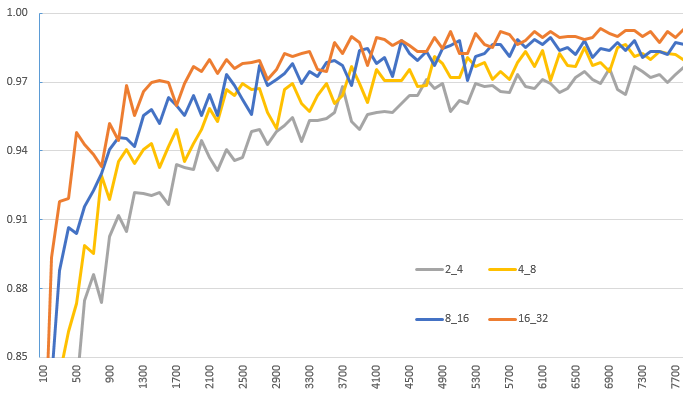
\includegraphics[width=1\textwidth]{Images/training_speed}
\end{figure}

The first perspective we explore is the speed of training phase, or rather how quickly the convolutional network learns from the example images. It is interesting to inspect this, because as we shall see in the graphics, in front of a greater number of features we find a more training speed. In other words it means: more features, more rapid learning.

Figure \ref{fig:training_speed} shows the first part of the training phase, about the first half. It allows us to focus on the most interesting part of the graphic for the analysis we are going to do.

Focusing on Figure \ref{fig:training_speed} we can clearly observe that more features imply a more rapid learning. We can notice this in two ways, two points of view.

Considering the same training value, e.g. $0.85$, we observe the following facts. that the model with fewer features (Model $2_4$) reaches the referring value in more than $500$ epochs.

\paragraph{Model 2\_4}

The TensorFlow model with fewer features reaches the referring value of training accuracy in more than $500$ epochs.

\paragraph{Model 4\_8}

Increasing the number of features we obtain the same training accuracy value of $0.85$ in about $350$ epochs.

\paragraph{Model 8\_16}

The model with $8$ and $16$ features on first and second convolutional layer reach that training accuracy value in about $200/250$ epochs.

\paragraph{Model 16\_32}

The last model with the higher number of features is the fastest, reaching the referring training accuracy value in about $150$ epochs.
\\
\\
Even without focusing on precise number of epochs, we can notice at a glance the slower and faster model. The same observations we just made, can be done considering a precise epoch during the first part of the training phase where the learning curve mainly grows.

\subsection{Training stability}

A second perspective in our analysis is the stability of training, particularly towards the end part of training phase. 

\begin{figure}
	\caption{Comparison of training stability of the four TensorFlow models with different number of features}
	\label{fig:training_stability}
	\centering
	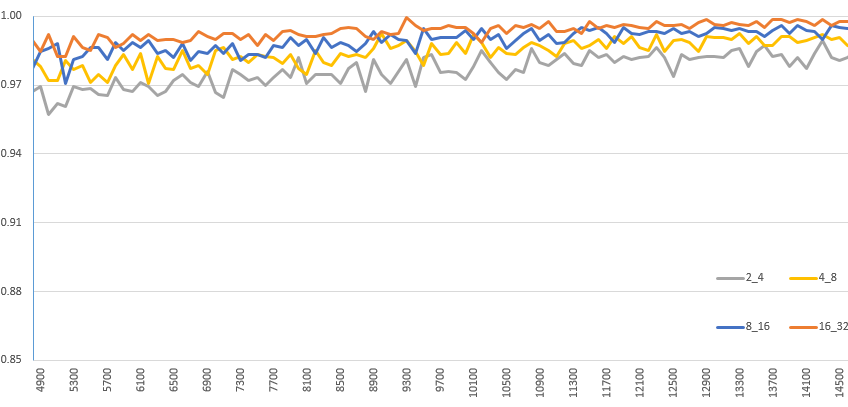
\includegraphics[width=1\textwidth]{Images/training_stability}
\end{figure}

\subsection{Training performance}

\begin{landscape}
	\begin{figure}
		\centering
		\caption{Comparison of training accuracy curves of the four TensorFlow models with different number of features}
		\label{fig:cfr_all}
		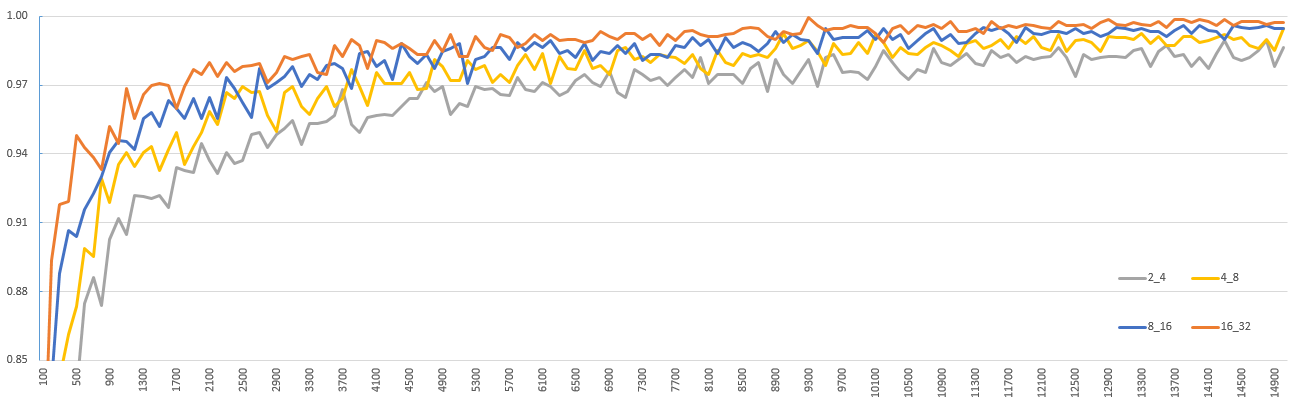
\includegraphics[width=1\textheight]{Images/cfr_all}
	\end{figure}
\end{landscape}

\subsection{Training duration}

\subsection{Influences of parameters on the network}

\section{Analysis of test accuracy}